% ============================================================
%  fig_prisma.tex
%  PRISMA 2020 Flow Diagram — standalone figure
%  Compile:  pdflatex fig_prisma.tex
%  Output :  figures/fig_prisma.pdf
%  Border  : 4pt (micro padding, matches table template)
% ============================================================
\documentclass[border=4pt]{standalone}

\usepackage[T1]{fontenc}
\usepackage[utf8]{inputenc}
\usepackage{mathptmx}
\usepackage[scaled=0.92]{helvet}
\usepackage{courier}
\renewcommand{\sfdefault}{phv}

\usepackage{amsmath}
\usepackage{tikz}
\usepackage{xcolor}

\usetikzlibrary{positioning, shapes.geometric, arrows.meta, fit, calc}

% ── colour palette ──────────────────────────────────────────
\definecolor{boxBg}    {RGB}{240,244,248}
\definecolor{boxBorder}{RGB}{ 90,120,160}
\definecolor{exclBg}   {RGB}{255,243,243}
\definecolor{exclBorder}{RGB}{200, 80, 80}
\definecolor{inclBg}   {RGB}{240,255,240}
\definecolor{inclBorder}{RGB}{ 60,160, 60}
\definecolor{phaseBg}  {RGB}{220,230,245}
\definecolor{inlineBg} {RGB}{230,230,230}

% ── node styles ─────────────────────────────────────────────
\tikzset{
  box/.style={
    rectangle, draw=boxBorder, fill=boxBg, rounded corners=3pt,
    line width=0.6pt, align=left, inner sep=6pt, font=\small
  },
  excl/.style={
    rectangle, draw=exclBorder, fill=exclBg, rounded corners=3pt,
    line width=0.6pt, align=left, inner sep=6pt, font=\small
  },
  incl/.style={
    rectangle, draw=inclBorder, fill=inclBg, rounded corners=3pt,
    line width=0.6pt, align=left, inner sep=6pt, font=\small
  },
  phase/.style={
    rectangle, draw=boxBorder, fill=phaseBg, rounded corners=3pt,
    line width=0.6pt, align=center, inner sep=6pt,
    font=\small\bfseries, minimum width=1.0cm
  },
  arr/.style  = {-{Stealth[length=5pt]}, line width=0.7pt, draw=boxBorder},
  arr2/.style = {-{Stealth[length=5pt]}, line width=0.7pt, draw=exclBorder,
                 dashed},
}

\newcommand{\code}[1]{\texttt{#1}}

% ============================================================
\begin{document}
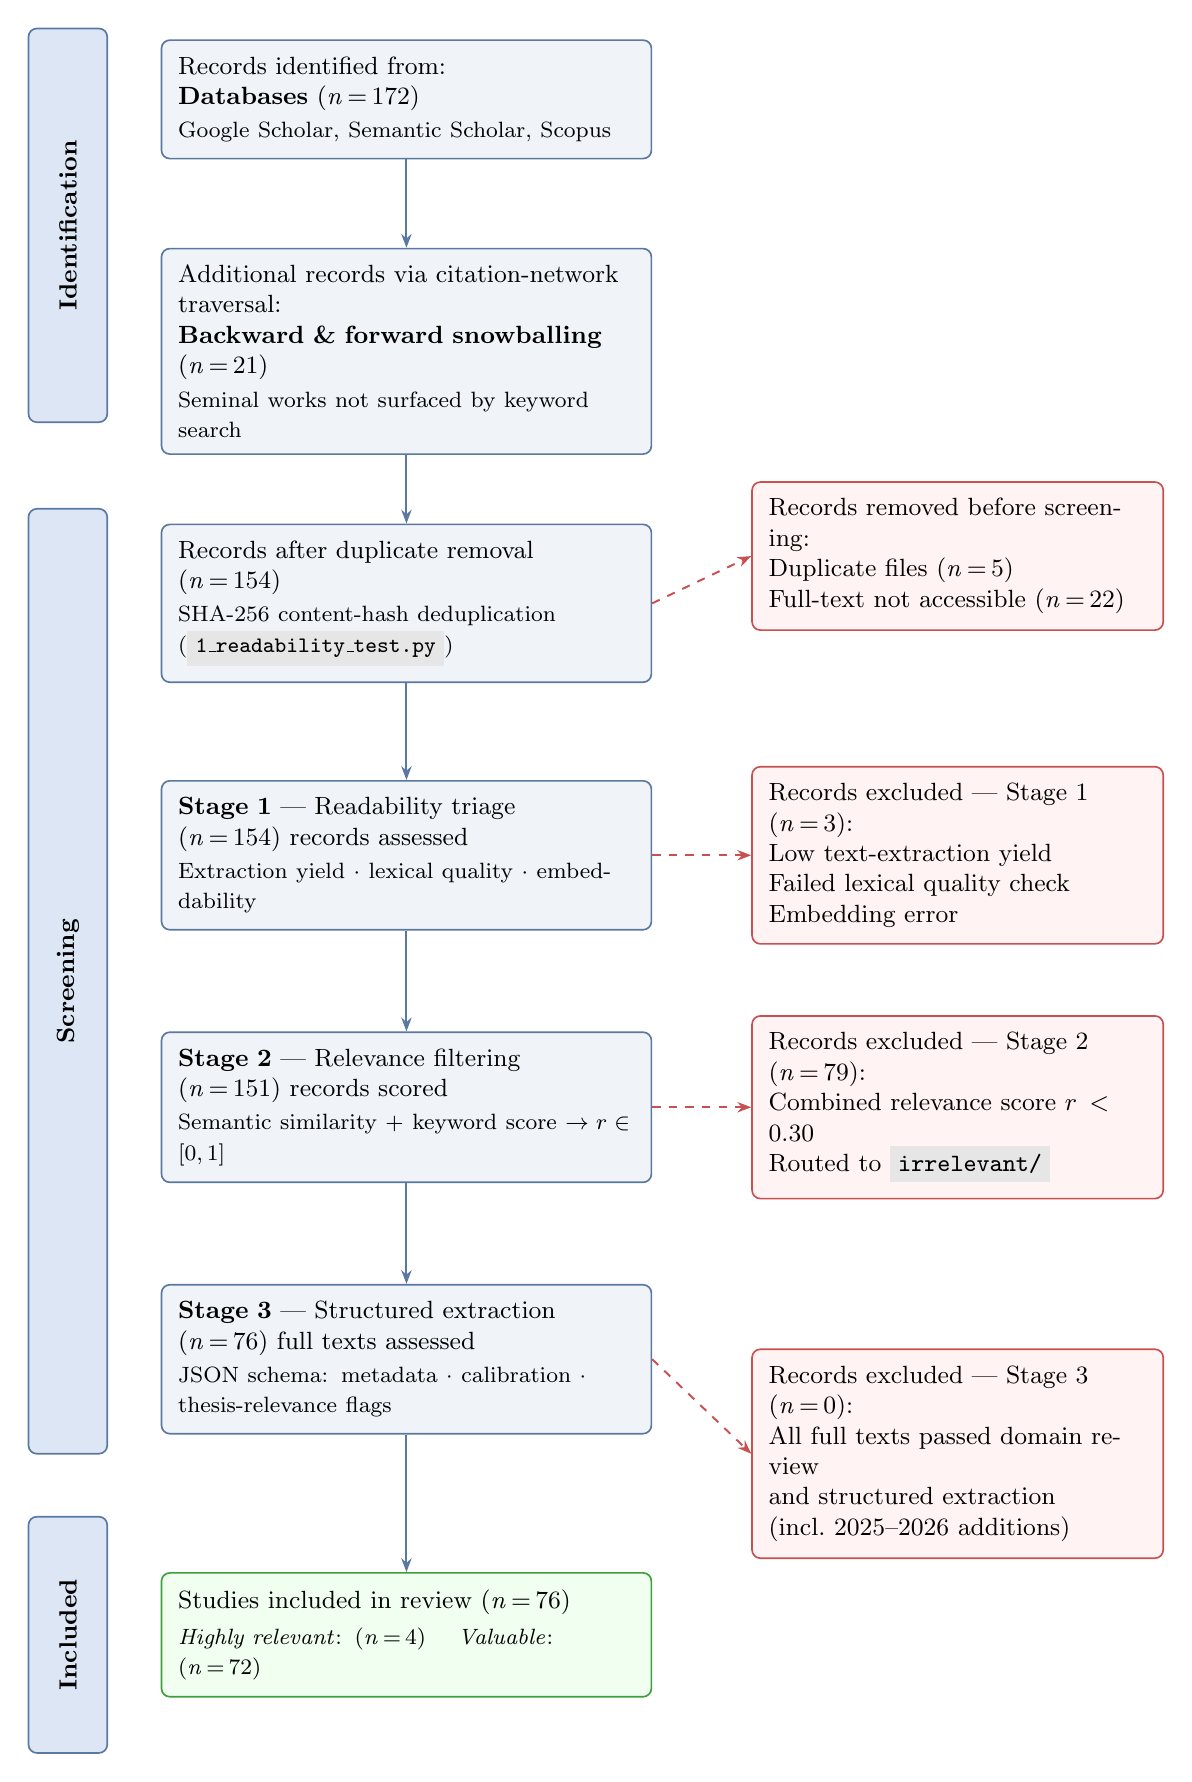
\begin{tikzpicture}

% ═══════════════════════════════════════════════════════════
%  IDENTIFICATION
% ═══════════════════════════════════════════════════════════
\node[phase, minimum height=5.0cm] (ph-id) at (-3.8, -1.6)
  {\rotatebox{90}{Identification}};

\node[box, text width=5.8cm] (id1) at (0.5, 0)
  {Records identified from:\\
   \textbf{Databases} (\textit{n}\,=\,172)\\[1pt]
   \footnotesize Google Scholar, Semantic Scholar, Scopus};

\node[box, text width=5.8cm] (id2) at (0.5, -3.2)
  {Additional records via citation-network traversal:\\
   \textbf{Backward \& forward snowballing} (\textit{n}\,=\,21)\\[1pt]
   \footnotesize Seminal works not surfaced by keyword search};

\draw[arr] (id1.south) -- (id2.north);

% ═══════════════════════════════════════════════════════════
%  SCREENING
% ═══════════════════════════════════════════════════════════
\node[phase, minimum height=12.0cm] (ph-sc) at (-3.8, -11.2)
  {\rotatebox{90}{Screening}};

\node[box, text width=5.8cm] (sc1) at (0.5, -6.4)
  {Records after duplicate removal\\
   (\textit{n}\,=\,154)\\[1pt]
   \footnotesize SHA-256 content-hash deduplication
   (\colorbox{inlineBg}{\texttt{\color{black}1\_readability\_test.py}})};

\node[excl, text width=4.8cm] (exc1) at (7.5, -5.8)
  {Records removed before screening:\\
   Duplicate files (\textit{n}\,=\,5)\\
   Full-text not accessible (\textit{n}\,=\,22)};

\draw[arr]  (id2.south) -- (sc1.north);
\draw[arr2] (sc1.east)  -- (exc1.west);

\node[box, text width=5.8cm] (sc2) at (0.5, -9.6)
  {\textbf{Stage 1} --- Readability triage\\
   (\textit{n}\,=\,154) records assessed\\[1pt]
   \footnotesize Extraction yield $\cdot$ lexical quality $\cdot$ embeddability};

\node[excl, text width=4.8cm] (exc2) at (7.5, -9.6)
  {Records excluded --- Stage 1 (\textit{n}\,=\,3):\\
   Low text-extraction yield\\
   Failed lexical quality check\\
   Embedding error};

\draw[arr]  (sc1.south) -- (sc2.north);
\draw[arr2] (sc2.east)  -- (exc2.west);

\node[box, text width=5.8cm] (sc3) at (0.5, -12.8)
  {\textbf{Stage 2} --- Relevance filtering\\
   (\textit{n}\,=\,151) records scored\\[1pt]
   \footnotesize Semantic similarity $+$ keyword score $\rightarrow r \in [0,1]$};

\node[excl, text width=4.8cm] (exc3) at (7.5, -12.8)
  {Records excluded --- Stage 2 (\textit{n}\,=\,79):\\
   Combined relevance score $r < 0.30$\\
   Routed to \colorbox{inlineBg}{\texttt{\color{black}irrelevant/}}};

\draw[arr]  (sc2.south) -- (sc3.north);
\draw[arr2] (sc3.east)  -- (exc3.west);

\node[box, text width=5.8cm] (sc4) at (0.5, -16.0)
  {\textbf{Stage 3} --- Structured extraction\\
   (\textit{n}\,=\,76) full texts assessed\\[1pt]
   \footnotesize JSON schema: metadata $\cdot$ calibration $\cdot$ thesis-relevance flags};

\node[excl, text width=4.8cm] (exc4) at (7.5, -17.2)
  {Records excluded --- Stage 3 (\textit{n}\,=\,0):\\
   All full texts passed domain review\\
   and structured extraction\\
   (incl.\ 2025--2026 additions)};

\draw[arr]  (sc3.south) -- (sc4.north);
\draw[arr2] (sc4.east)  -- (exc4.west);

% ═══════════════════════════════════════════════════════════
%  INCLUDED
% ═══════════════════════════════════════════════════════════
\node[phase, minimum height=3.0cm] (ph-inc) at (-3.8, -19.5)
  {\rotatebox{90}{Included}};

\node[incl, text width=5.8cm] (inc1) at (0.5, -19.5)
  {Studies included in review
   (\textit{n}\,=\,76)\\[2pt]
   \footnotesize \textit{Highly relevant}: (\textit{n}\,=\,4)
   \quad \textit{Valuable}: (\textit{n}\,=\,72)};

\draw[arr] (sc4.south) -- (inc1.north);

\end{tikzpicture}
\end{document}